\documentclass{chi2009}
\usepackage{times}
\usepackage{url}
\usepackage{graphics}
\usepackage{color}
\usepackage[pdftex]{hyperref}
\usepackage{graphicx}
\usepackage{tabularx}
\usepackage{booktabs}

\newcommand{\docTitle}{Improving Usability of the Linux Kernel Configuration Tools}
\newcommand{\docKeywords}{usability, linux, kernel, configuration}

\hypersetup{%
pdftitle={\docTitle},
pdfauthor={Kacper Bak},
pdfkeywords={\docKeywords},
bookmarksnumbered,
pdfstartview={FitH},
colorlinks,
citecolor=black,
filecolor=black,
linkcolor=black,
urlcolor=black,
breaklinks=true,
}
\newcommand{\comment}[1]{}
\definecolor{Orange}{rgb}{1,0.5,0}
\newcommand{\todo}[1]{\textsf{\textbf{\textcolor{Orange}{[[#1]]}}}}
\newcolumntype{S}{>{\centering\arraybackslash} m{.4\linewidth} }

%
%  Convenience commands for references
%
\newcommand{\secref}[1]{Section~\ref{sec:#1}}
\newcommand{\tabref}[1]{Table~\ref{tab:#1}}
\newcommand{\figref}[1]{Fig.\,\ref{fig:#1}}
\newcommand{\Figref}[1]{Figure\,\ref{fig:#1}}
\newcommand{\eqaref}[1]{equation~\eqref{eq:#1}}
\newcommand{\defref}[1]{Definition~\eqref{def:#1}}
\newcommand{\lemref}[1]{Lemma~\eqref{lem:#1}}
\looseness=-1

\pagenumbering{arabic}  % Arabic page numbers for submission.  Remove this line to eliminate page numbers for the camera ready copy

\begin{document}
% to make various LaTeX processors do the right thing with page size
\special{papersize=8.5in,11in}
\setlength{\paperheight}{11in}
\setlength{\paperwidth}{8.5in}
\setlength{\pdfpageheight}{\paperheight}
\setlength{\pdfpagewidth}{\paperwidth}

% use this command to override the default ACM copyright statement 
% (e.g. for preprints). Remove for camera ready copy.
\toappear{Submitted for CS 889 - Open Source Usability.}

\title{\docTitle}
\numberofauthors{2}
\author{
  \alignauthor Kacper Bak\\
    \affaddr{Generative Software Development Lab}\\
    \affaddr{University of Waterloo, Canada}\\
    \email{kbak@gsd.uwaterloo.ca}
  \alignauthor Karim Ali\\
    \affaddr{PLG Group}\\
    \affaddr{University of Waterloo, Canada}\\
    \email{karim@uwaterloo.ca}
}

\maketitle

\begin{abstract}
Tailoring a Linux kernel to one's needs has been one of the most cumbersome tasks a GNU/Linux user can do. There have been many attempts to overcome this
problem by introducing smarter configuration tools. Those tools, however, still lack some important features which discourages users from using them. In this
project, we address the problem of usability of the Linux kernel configuration tools. We identify the major usability issues with current tools, propose a
better user interface and evaluate it on a group of Linux enthusiasts.
\end{abstract}

\keywords{\docKeywords} 

\category{H.5.2}{Information Interfaces and Presentation}{Miscellaneous}%[Optional sub-category]

\section{Introduction}

GNU/Linux is a free operating system with Linux as its kernel. The Linux kernel\footnote{Available at: \url{http://www.kernel.org/}} is a mature and very complex piece of software. It has been developed by thousands of programmers led by Linus Torvalds since 1991. The kernel supports a variety of computer architectures, network protocols, thousands of drivers, and many debugging options.

The structure of the kernel is very modular such that each user can tailor it to her particular needs and specific hardware. Recent research
\cite{she:kernel:2010} has shown that the whole kernel is composed of almost 5500 features, of which 89\% are user-selectable. Thus, the variation space is huge
and the configuration process requires a broad computer knowledge. Users can configure the kernel either by manually editing the \textsf{.config} file or by
using some configuration tool (i.e. \textsf{menuconfig, xconfig, gconfig}). The first option is discouraged, because it is very error-prone due to lack of
automated constraint validation/propagation. Using a configurator is a better solution, but it is still a laborious process.

Existing configuration tools have been evolving for over a decade, but the progress is reasonably slow compared to other parts of the kernel. Usability seems to
have a low priority on developers' task lists. To address this issue, we started a course project aimed at making the configuration process easier and more
intuitive for Linux enthusiasts. The project went through three major stages as shown in Figure \ref{fig:flow}. First, we carried out an initial user study
to identify major usability issues of the current Linux kernel configuration tools. We then proposed some alternative mockup designs based on the feedback we
got from the participants. Second, we carried out a user study to get comments and constructive feedback on the various design mockups we had for our tool
prototype. According to the feedback, we reflected user suggestions and remarks in the implementation of the prototype. Finally, we did a final user study to
evaluate our prototype and compare it to \textsf{xconfig}. General reactions of the test group were positive and participants saw the new tool as an improvement
over the standard tools. We believe that our findings will help in creating better configuration applications not only for the Linux kernel, but also for other
kinds of variability models.

\begin{figure*}[!t]
 \centering
 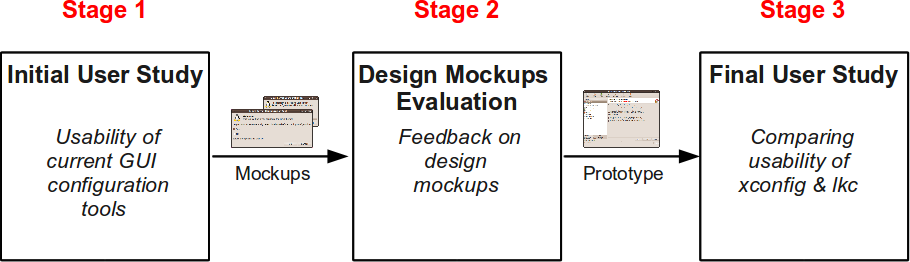
\includegraphics[scale=0.5,keepaspectratio=true]{figs/flow}
 \caption{Different project stages}
\label{fig:flow}
\end{figure*}

The rest of this paper is organized as follows. We first describe the problem domain. We then present the results of our initial user studies of current tools
and design mockups. Afterwards, we explain how we reached the design of our tool prototype. We then present the results of our final user study to evaluate our
tool in comparison to \textsf{xconfig}. We then discuss possible future work. Finally, we present some related work and end the paper by some concluding
remarks.

\section{Problem}\label{sec:problem}

% motivation
People configure operating system kernels for several reasons. Usually, they want to customize kernels to specific hardware or to particular needs. This
scenario is very common in embedded systems such as network routers, where hardware resources are very limited. By carefully selecting options, one can improve
system stability or functionality. Although many configuration options are related with hardware and device drivers, there is also a large group of options that
change the way operating system works. A good example is the \textit{preemptible scheduler} that makes Linux a soft real-time
operating system. Such a scheduler is desirable for digital signal processing; e.g. for recording and transforming signal from the guitar.

The majority of users configure kernels without even realizing this fact. We distinguish between two types of kernel configuration: static and dynamic. In the
former method, software is customized before compilation so that only chosen pieces of code are compiled. It results in a smaller program footprint and faster
compilation. On the other hand, the latter configuration requires more effort because any additional piece of software has to be compiled separately. In many
modern distributions users are provided with fully functional kernels, which they do not have to compile themselves. Instead, they dynamically customize the
software by loading relevant modules. The disadvantage of the second method is that preparing such a big kernel takes a lot of time and resources. Furthermore,
it is infeasible to apply it to embedded systems.

% current sw
Regardless of the configuration type, there is still need to customize the software. Although this task can be done manually, most users prefer to use automated
and intuitive tools that could guarantee that the system works properly. Unfortunately, the software currently used for kernel configuration is neither fully
automated nor easy to use. In addition, static and dynamic configuration are two separate mechanisms and are supported by completely different programs. Static
configuration is done by the Linux Kernel Configurator, while dynamic configuration is done by adding or removing compiled modules using other tools (e.g.
\textit{modprobe}). In our opinion, the two worlds can be merged to provide a single user interface.

Linux kernel configurators are targeted to advanced users. Some kernel developers believe that kernel should be configured only by experienced users
\cite{kernel:aunt:2002}. While this statement might be true, there are still lots of Linux novice or less experienced users who want to learn how to configure a
kernel or need to compile/load a particular driver. Currently, there are millions of web pages describing how to configure and compile the Linux kernel. Novice
users are often overwhelmed by the number of available options and required knowledge. To understand the current challenges of configurating a kernel, we
carried out an initial study on a group of Linux users.

\section{User Studies}\label{sec:userstudies}

\subsection{Initial User Study}
% initial study
In the study, six participants were asked to statically configure the Linux kernel for a popular laptop for typical home or office use. They used the standard
\textsf{xconfig} tool that comes with the Linux kernel. \textsf{xconfig} presents a list of options in a tree structure composed of categories and options. A
person succeeded if the new kernel was ready to play music and movies, connect to Ethernet, use WiFi, memory cards, USB devices, Bluetooth, and CD/DVD. This
scenario seems reasonable, because in many Linux distributions users have to fine-tune their configurations to make the whole system work as expected. None
of the subjects succeeded in completing the task without asking us for further assistance. We observed many problems that people faced during the configuration
process. It is worth noting that our participants had previous experience with Linux, and claimed to be advanced computer users. During the study, we were also
interested in how they use curret kernel configuration tools (e.g. \textsf{xconfig}), and how people configure software in general. Our findings are summarized
in several categories:

\begin{description}
  \item[Menu hierarchy]
All participants had problems with selecting drivers for the laptop's hardware. First of all, the tool showed the whole menu hierarchy, and people said they
were overwhelmed by thousands of options. Several of them started by collapsing all menus such that only top-level categories were visible. Furthermore, the
tree/sub-tree relationship was confusing. It was unclear whether marking the checkbox beside a parent option implies the selection of the required
functionality or additional sub-options should be selected as well. To some, even such a basic action such as checking an option was confusing. Besides the
familiar empty and filled checkboxes, the tool showed some boxes with dots inside. This meant that the option will be compiled, but as a dynamically loadable
module.

  \item[Option names and descriptions]
Cryptic names were another source of problems. The existing infrastructure uses option names that make sense to programmers and kernel hackers, but are hard to
understand for less experienced users. Unfortunately, the descriptions were not very helpful since they often explained implementation details instead of
end-user functionality. Participants expected to see what an option means to them, and whether the device driver is appropriate for their hardware. In many
cases, their expectations were not met.

  \item[Searching]
The huge hierarchy of options and cryptic names make it very hard to find a particular feature. All participants used the search option in \textsf{xconfig}.
Searching worked very poorly since feature descriptions were not included in the search space of the tool. People expressed their frustration and often used
Google to match modules with hardware, and later select the module in \textsf{xconfig}. Google was also used to find a list of the drivers required by the
laptop. For all users, querying a web search engine was easier than running system tools to discover hardware devices.

  \item[Configuration]
We carefully observed how users used current tools to configure a large piece of software. Most of them were jumping between different categories as they tried
to locate modules. One person, who had experience with kernel configuration tools, started the \textsf{menuconfig} program which performs wizard-like
configuration. The problem with this tool was that the user could not jump between categories, and had to answer many irrelevant questions. After a while, the
participant switched to \textsf{xconfig}. Users had problems with selecting appropriate device drivers. When they were unsure about which module to choose, they
selected all the modules that seemed relevant. 
\end{description}

% conclusions

The initial study was a necessary step to discover user expectations and needs. It led us to the following conclusions:
\begin{enumerate}
\item The menu hierarchy should be as simple as possible. There are far too many options that could be reduced automatically if the configuration tool targeted
a specific user group (novice and intermediate users) and had good reasoning capabilities.
\item Feature names and descriptions should reflect end-user functionality instead of low-level details.
\item Powerful searching capabilities are crucial as the number of configuration options grows.
\item Automatic hardware detection and kernel autoconfiguration is important since the majority of kernel options are related to hardware drivers.
\end{enumerate}

The aforementioned problems can be fixed by improving the application's backend and creating a more intuitive user interface. Our project focuses on
constructing a GUI that would be intuitive, simple and targeted to a specific group of users (novice and intermediate users).


\subsection{Design Mockups Evaluation}
We decided that our tool should be built to help novice and intermediate Linux users configure a Linux kernel without burdening them with many of the unncessary
details involved in such a process. We designed several mockups that reflect this vision for the tool. Initially, we thought that once the tool is launched, it
should first fetch the current Linux kernel configuration, then detect the currently connected hardware. A dialog box (splash screen) should be shown to the
user at that time to show the progress of these processes. Figure \ref{fig:splash} shows four different mockups for that dialog box.

\begin{figure*}[!t]
 \centering
\begin{tabular}{SS}
 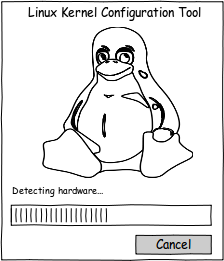
\includegraphics[scale=0.5,keepaspectratio=true]{figs/splash-big} & 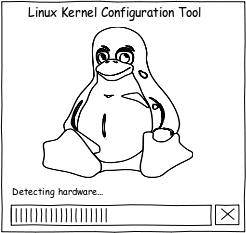
\includegraphics[scale=0.5,keepaspectratio=true]{figs/splash-bigico} \\
 (a) & (b) \\
 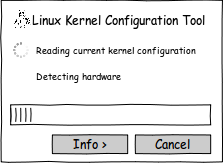
\includegraphics[scale=0.5,keepaspectratio=true]{figs/splash-readingcurrent} &
 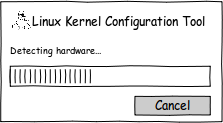
\includegraphics[scale=0.5,keepaspectratio=true]{figs/splash-standard} \\
 (c) & (d) \\
\end{tabular}
\caption{Splash screen design mockups}
\label{fig:splash}
\end{figure*}

We carried out a second user study that included six participants. The aim of this study was to show the participants those mockup designs and get feedback from
them regarding which aspects in those designs were appealing to them, and which were not. That study led us to draw the following conclusions:
\begin{enumerate}
 \item Users always like to know what is going on. In other words, they did care about getting more information about what the tool is doing while the progress
bars are being filled up.
 \item Users appreciate access to more information, but prefer such information to be displayed only when requested rather than by default.
 \item It is highly desirable to have the tool report any crashes that occur during the hardware detection process.
\end{enumerate}

In addition to showing the participants of this user study some mockup designs for the splash screen of our tool, we also showed them some mockup designs
for the application itself. Figure \ref{fig:lkc-tool} shows the various mockups that were shown to the participants of this study. The feedback we got from the
users allowed us to deduce the following:
\begin{enumerate}
 \item Almost all users liked having helpful descriptions for the various kernel features they can select.
 \item Easy navigation through the various categories of features was also on top of thier desirable design features.
 \item The fewer the number of categories were, the easier it was for the users to find features.
 \item Some users did not like the wizard-based design (Figure \ref{fig:lkc-tool}d) because it did not offer easy navigation through features and did not
provide a search feature.
 \item Most users liked the fact that they were presented by a summary of the configuration file at the end of the process with the ability to review it and
maybe modify it before quitting the application.
 \item Although many users were not in favor of the wizard-based design, they did like the question format that was presented in that design. The reason is
that it gave them a better understanding of the effect of selecing/deselecting features.
\end{enumerate}

\begin{figure*}[!t]
 \centering
\begin{tabular}{SS}
 \multicolumn{2}{c}{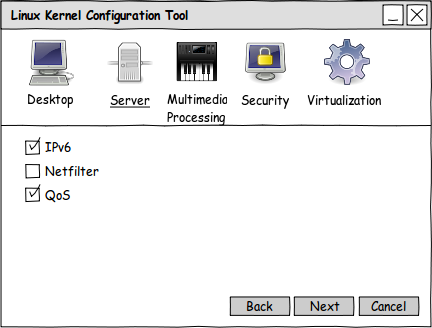
\includegraphics[scale=0.5,keepaspectratio=true]{figs/lkc-barwithicons}} \\
 \multicolumn{2}{c}{(a)} \\
 \multicolumn{2}{c}{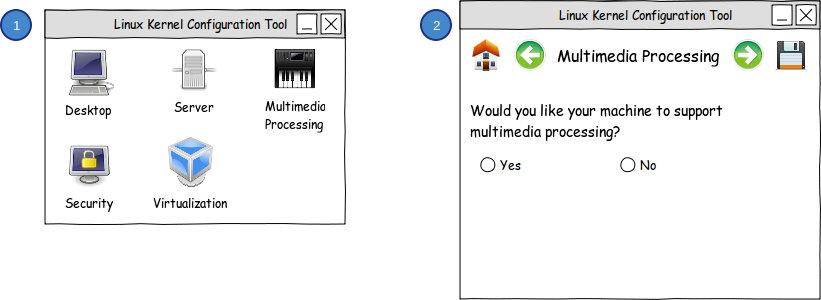
\includegraphics[scale=0.5,keepaspectratio=true]{figs/lkc-browser}} \\
 \multicolumn{2}{c}{(b)} \\
 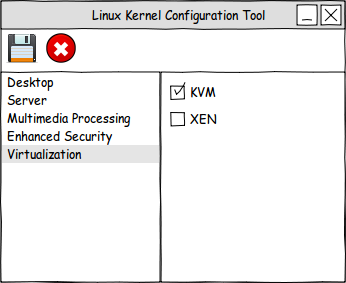
\includegraphics[scale=0.5,keepaspectratio=true]{figs/lkc-tree} &
 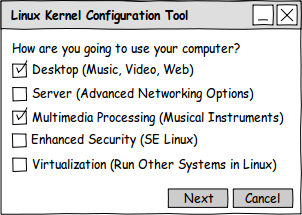
\includegraphics[scale=0.5,keepaspectratio=true]{figs/lkc-wizard} \\
 (c) & (d) \\
\end{tabular}
\caption{\textsf{lkc} tool design mockups}
\label{fig:lkc-tool}
\end{figure*}

\section{Linux Kernel Configuration Tool}\label{sec:lkc}

\subsection{Splash Screen}
According to the feedback we got from our second user study, we designed the splash screen of our prototype as shown in Figure \ref{fig:splash-final}. In the
prototype of the splash screen, the user will be asked whether she wants to detect the current hardware or not. If she answers yes, she will be presented with
the dialog shown in Figure \ref{fig:splash-final}a. The list of tasks along with the progress bar gives the user an idea about the task that the tool is
currently doing. Thus, we satisfy the first conclusion. If the user would like to get more information, she can click on the \textit{Information} button. The
user will then be presented by a scrollable text area that shows the current action (e.g. Detecting device ... dev 40). This text area is hidden by default to
satisfy the second conclusion. In case of a crash, the text area will show the user more information about the possible causes of the crash and the progress of
the tool so far. Therefore, the design satisfies the third conclusion.

\begin{figure*}[!t]
 \centering
\begin{tabular}{SS}
 \begin{tabular}{c}
  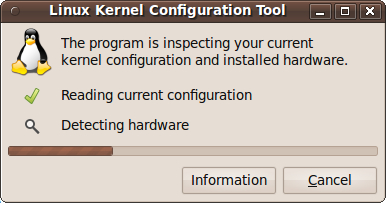
\includegraphics[scale=0.5,keepaspectratio=true]{figs/splash-final1} \\
  (a) \\
 \end{tabular}
  & 
\begin{tabular}{c}
  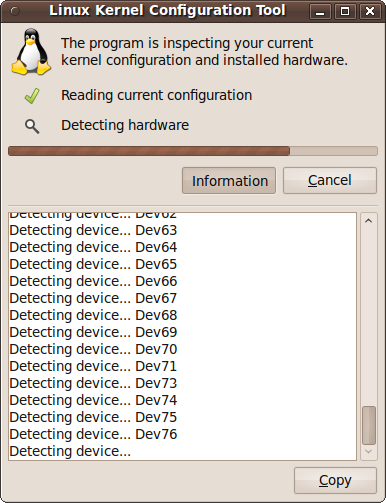
\includegraphics[scale=0.5,keepaspectratio=true]{figs/splash-final2} \\
  (b) \\
 \end{tabular}
\end{tabular}
\caption{Splash screen prototype}
\label{fig:splash-final}
\end{figure*}

\subsection{\textsf{lkc} Tool}
Based on our conclusions from the second part of our second user study, we designed a prototype for the \textsf{lkc} as shown in Figure \ref{fig:lkc-final}. The
figure shows various steps during the process of a configuring a Linux Kernel. The design of the prototype is a mixture between the tree-based design (Figure
\ref{fig:lkc-tool}c) and the wizard-based design (Figure \ref{fig:lkc-tool}d). The rationale behind this mixture is that we tried to get the best out of the two
designs because they were the two most appreciated designs among the participants of our second user study. Having such design allows users to go through the
step-by-step configuration process that the wizard design provides. In the meanwhile, users can still enjoy the comfort of free navigation through the various
categories of features using the left panel. Therefore, we satisfy the second conclusion. We also tried to provide the users with as few categories as possible
and label them with less cryptic names than the ones used in current Linux kernel configuration tools (e.g. \textsf{xconfig}). No matter how the user navigates
through the categories of features, she will always be presented with a question related to the currently selected viewed category. The answer to this question
reflects on enabling the related kernel features accordingly. Therefore, the user does not have to directly deal with setting/unsetting kernel features, but
rather answering questions that better match her usage of the machine she wants to compile this kernel for. Thus, the design satisfies our sixth conclusion. The
menu bar at the top of the application window provides the user with fast access to tasks like:
\begin{enumerate}
 \item Starting a new configuration process.
 \item Opening a previously saved configuration file into the tool.
 \item Saving the current configuration to a file on disk.
 \item Keyword searching within the feature names, descriptions and help text.
 \item Switching to an advanced mode, where the user will be able to use \textsf{xconfig} instead of our to complete the configuration.
 \item Navigating through the categories of features presented in the left panel.
\end{enumerate}

We also added a panel that shows the statistics of the kernel that will be compiled using the currently selected features. Statistics include:
\begin{enumerate}
 \item Progress of the current configuration session.
 \item Total kernel size based on the currently selected set of features.
 \item Total number of features.
 \item The stability of the kernel to be compiled by the generated configuration file. This is based on the least stable selected kernel feature.
\end{enumerate}

In addition to statistics about the whole kernel, the prototype also shows information about each feature when selected. The information is about the effect
of selecting this feature on the total kernel size, and how stable that feature is. Moreover, the prototype shows a panel at the very bottom that lists all the
conflicts that are currently found in the configuration. However, this feature has not been implemented yet due to time constraints.

The first step that the user will encounter using our tool is the welcome screen (Figure \ref{fig:lkc-final}a) where there is an explanation of how the tool
can be used to configure a Linux kernel. The explanation includes some notes about the defaults options, how to navigate through categories, and what to do
when the user is done. Therefore, we satisfy our first conclusion. Depending on the selections that the user makes in the subsequent screens, some categories of
features (from the left navigation panel) will be skipped by the \textit{Next} button because they are irrelevant to the user's choices. However, if the user
thinks otherwise and would like to change some of the features in such categories, she can navigate to any of those categories using the left navigation panel.
Once the user feels comfortable with the configuration, she can save the configuration to a file on disk using the \textit{Save} button in the menu bar at the
top. Alternatively, she can go on with all the steps, then get a summary of the configuration options she selected before saving the configuration to a file on
disk. Thus, the design satisfies our fifth conclusion.

\subsection{Implementation}
The implementation of our \textsf{lkc} tool prototype seperates the graphical user design from the code that actually manages that design. We used Glade
\cite{glade:2010}, a rapid application development tool for GTK+ and GNOME, to design the interface of the prototype. Glade is Free Software released under the
GNU GPL License, which perfectly goes along with the topics we discussed in class. Glade has many language bindings making it easy to re-use the same Glade
design with different languages. We chose to work with the Java bindings for Glade \cite{java-gnome:2010} because we are more familiar with that language which
makes the process of protoyping easier and faster. We used Eclipse \cite{eclipse:2010} as our integrated development environment (IDE) to produce the Java code
that will manipulate the interface designed with Glade.

All the work we have done so far for this project including: source code files, mockup designs, reports, presentation and this report are avialable online at
our github repository \cite{git-lkc:2010}.

\begin{figure*}[!t]
 \centering
 \begin{tabular}{SS}
 \begin{tabular}{c}
  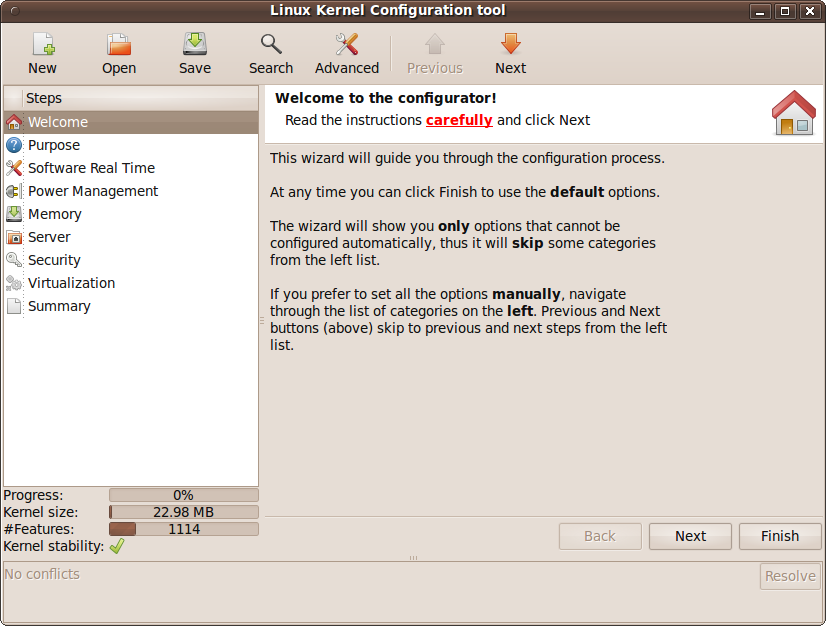
\includegraphics[scale=0.25,keepaspectratio=true]{figs/lkc-final1} \\
  (a) \\
 \end{tabular}
  & 
\begin{tabular}{c}
  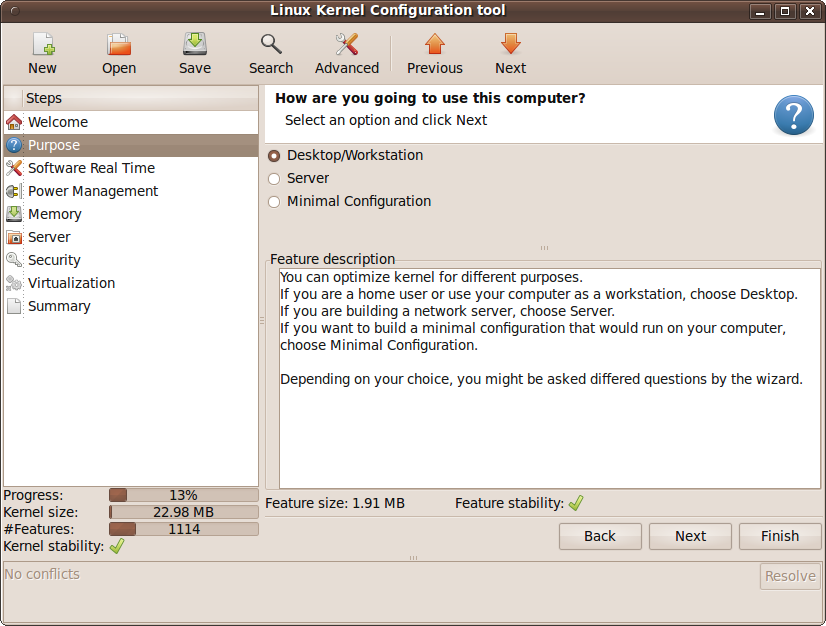
\includegraphics[scale=0.25,keepaspectratio=true]{figs/lkc-final2} \\
  (b) \\
 \end{tabular} \\
 \begin{tabular}{c}
  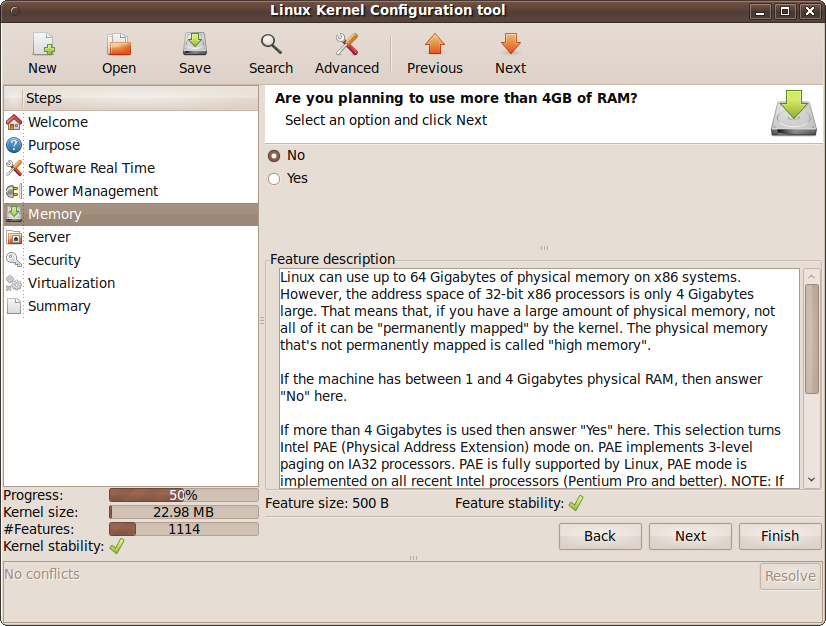
\includegraphics[scale=0.25,keepaspectratio=true]{figs/lkc-final3} \\
  (c) \\
 \end{tabular}
  & 
\begin{tabular}{c}
  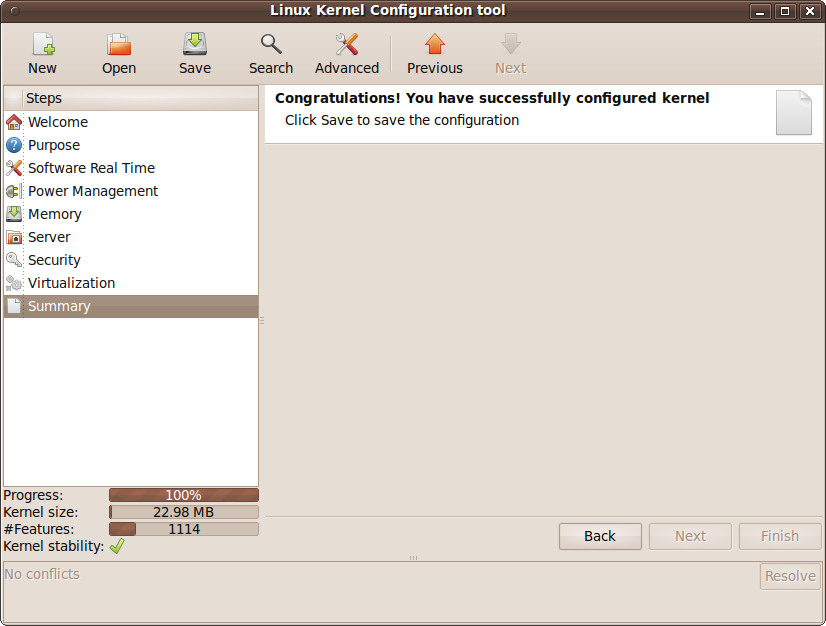
\includegraphics[scale=0.25,keepaspectratio=true]{figs/lkc-final4} \\
  (d) \\
 \end{tabular}
\end{tabular}
\caption{\textsf{lkc} tool prototype}
\label{fig:lkc-final}
\end{figure*}

\section{Evaluation}\label{sec:evaluation}
We carried out a final user study to evaluate the usability of our tool prototype and compare it to \textsf{xconfig}. We had two option to do this study. The
first option was to provide the participants with our prototype, a list of desired kernel features and a list of hardware to be supported. We then ask the users
to configure a kernel using our prototype to support such configuration. The disadvantage of this approach is that we will not get to compare our prototype
with the currently available kernel configuration tools (e.g. \textsf{xconfig}). The other approach was to provide the participants of our study with both
tools, our prototype and \textsf{xconfig}. We then provide them with the same information as in the first option. However, this time we can compare the
usability of our prototype with that of \textsf{xconfig}. We opted for the second approach.

\subsection{Findings}
\subsubsection{\textsf{xconfig}}
In general, users complained about having too many options to configure. The way the options are categorized and laid out confused them even more. In addition,
users did not find the searching capabilities in \textsf{xconfig} to be usefull at all. The reason is that the search tool only matches substrings in the
configuration parameter names ignoring the description and help text provided. Some users resorted to Google instead to find the which kernel parameters they
are after.

Hardware configuration was also a consistent source of frustration to users. It was always hard to find drivers in the kernel options. Moreover, it was
difficult to match hardware with kernel module names.

\subsubsection{\textsf{lkc tool prototype}}
The positive feedback we got from users was that our prototype is definitely an improvement compared to \textsf{xconfig}. Users had various reasons to make such
a statement. In general, comments stated that the prototype is simple, intuitive and easy to use. Additionaly, users really appreciated the two-way navigation:
free navigation through the left panel, and wizard-based navigation through \textit{Back/Next} buttons. Users also appreciated the statistics panel because it
gave them an idea of how their current selections reflect on the overall status of the kernel that will be configured using the generated configuration file.
Finally, hiding unnecessary details and not overwhelming users with an explosion of features was another source of appreciation.

On the other hand, some users experienced difficulties using our prototype. One user did not know the meaning of \textit{features} in the statistics panel. Two
users did not quite understand what \textit{stability} means in our prototype. The option \textit{Minimal configuration} was rather confusing for one of our
users. Finally, one of the users commented on the fact that the study we carried on was biased because it was easy to accomplish the task just by answering the
questions provided by the tool.

\subsection{Threats to Validity}

\subsubsection{External Validity}
We could only get six users to participate in our final user study. This might not be a good sample of the whole population. Therefore, it would be great to
have the opportunity to include more participants in that study to be able to generalize our conclusions.

\subsubsection{Internal Validity}
Opting for the second approach was risky in the sense that we felt it will be biased to our application. The reason is that in our prototype if users have a
list of desired kernel features, they can easily reach to it by browsing the categories. However, that is not the case for \textsf{xconfig} where users will
have to search for such features and enable them. To reduce such bias, we decided to provide the users with a hypothetical scenario of a user and how he
actually uses his machine, along with the hardware configuration of that machine. We then asked the users to help that person out by configuring a kernel that
will support his machine usage and hardware.

Although this scenario seems to reduce the bias as we expected, one user did note that the study was biased to our tool. However, from the comments of that
user we got that the reason behind such claim is the question format followed by our tool. As we previously mentioned in Section \ref{sec:userstudies}
question-based configuration usually gives the user a better understanding of the whole process.

\section{Future Work}\label{sec:futurework}
We got a very rich feedback from the participants of our final user study about the design of our prototype. Implementing some of those suggestions would add
more value to the prototype. The design suggestions include the following:
\begin{enumerate}
 \item Provide progressive disclosure to accomodate both advanced and less experienced users.
 \item Have the ability to re-detect hardware.
 \item Provide info about detected hardware.
 \item Change the position of the \textit{Save} button.
 \item Always enable \textit{Finish} button. When clicked, it should show a dialog with three options: \textit{Save \& Quit}, \textit{Save}, and
\textit{Cancel}.
 \item Move \textit{Previous/Next} tool bar buttons closer to the left panel because they are ways of controlling the navigation through it.
 \item Keep history.
 \item Resolve conflicts.
\end{enumerate}

Finally, it would be interesting to have a fully functional application with all the desired features implemented and use it for real life scenarios and get
feedback from the FOSS community about the feature set it provides, and its design.

\section{Related Work}\label{sec:relatedwork}
% literature review

All the Linux kernel configuration tools are front-ends built on top of a single engine called Linux Kernel Configurator (LKC). LKC analyzes kernel variability
and supports users during the configuration stage. Internally, LKC uses the KConfig language to represent variability and dependencies among features.
A well-understood feature model for the Linux kernel features should always yeild a practically well-crafted variability model for the Linux kernel
\cite{sincero:lkc:2008,she:kernel:2010}. In contrast with formal feature models, LKC is not supported by any formal reasoning engine (e.g. SAT-solver). This is
a serious problem, because users can unconsciously create wrong configurations while having no clue why a particular configuration does not work. The Linux
kernel community can benefit from adopting well-researched feature models which can make their tools more reliable and usable.

Improvements of kernel configuration tools were already introduced in 2002 when Eric S. Raymond presented the CML2 configuration system
\cite{raymond:cml2:2000}. It allows for effective reasoning on kernel feature model and also provides progressive-disclosure. There was a long debate and flame
war about using that system \cite{kerneltrap:linux:2002}. It was rejected for various reasons, such as Eric S. Raymond's attitude, its Python dependency, its
complexity, and its radically new design. Many Linux developers prefer to introduce gradual updates to the kernel instead of applying one big patch.

\textit{eCos}~\cite{veer:ecos:2000} is an open source real-time operating system. It was designed to be configurable and to run on a wide variety of hardware
platforms. Similar to the Linux kernel, eCos comes with configuration tools. The eCos configurator is much more advanced, and arguably better-thought, since
it can detect conflicting options and guide users to resolve them. The eCos Configuration Tool has many features, but presents them in a single tree hierarchy.
In comparison with our tool, eCos features are often low-level and very technical. Additionaly, the eCos Configuration Tool does not offer any wizard so users
must have expertise if they want to skip irrelevant categories.

Hardware autodetection and kernel configuration is a recurring problem \cite{debian:config:2010,soft32:config:2007}. Many users complain about the lack of it.
The situation is slowly improving as developers added the \textsf{localmodconfig} \footnote{More info at: \url{http://bit.ly/cPgq8R}} target to Linux-2.6.32.
The command detects current kernel configuration and applies the same options to the new kernel. It is a step ahead, but the tool is very simplistic and assumes
that all the required modules are already loaded. For example, if a computer has built-in Bluetooth, but the module is not loaded, the new kernel will not
support the Bluetooth device. Furthermore, the autoconfiguration script offers a very coarse level of options' granularity. For example, if a computer has one
sound card, such as Intel HD Audio, the script will select all available sound card drivers and all Intel HD Audio modules. The autoconfiguration tool reads
configuration of the running kernel instead of detecting the actual hardware. For example, for a laptop with a Core Duo 2 processor, it selects the 686
processor in the new kernel, because that processor is selected in the running kernel.

Debian GNU/Linux device driver check \& report \cite{muto:check:2010} is an interesting project that helps with matching kernel modules with hardware. It reads
output of \textsf{lspci} command, and returns a list of driver names. The project is in fact a big database that stores user's knowledge about the hardware. It
could be utilized by the configurator to automatically select relevant modules if autodetection fails. Currently, the database aggregates only information about
PCI devices, and does not support ISA, USB, IEEE1394 or other hardware.

System configuration is a necessary, but difficult process. Our tool tried to simplify it by asking as few questions as possible and targeting a specific group
of users (novice and intermediate Linux users). \cite{spillers:config:2010} suggests a similar approach. The author goes even further saying that software shall
configure itself automatically. However, making a configuration-free kernel on any platform seems rather impossible due to requiring extra knowledge that is not
included in configurators.

% OSS usability
Free and Open Source Software usability has recently got attention from both academia and the FOSS community. Several researchers
\cite{nichols:usability:2003, andreasen:usability:2006} tried to understand why FOSS developers traditionally gave low priority to usability issues. Other work
studied particular projects such as Apache \cite{mockus:apache:2000} or Mozilla \cite{mockus:mozilla:2002} to learn about social interactions, FOSS culture and
the way the software is developed. Cooperation of the two communities allows the usability community to understand FOSS developers' attitudes. FOSS community,
on the other hand, benefits from learning usability-related knowledge and evaluation techniques.

\section{Conclusion}\label{sec:conclusion}
The Linux kernel is a complex piece of software that is highly customizable which might overwhelm novice and intermediate users. Currently available tools do
not provide an adequate solution for them. The results of our user studies show that users (even advanced users) prefer to have some features available in a
typical Linux kernel configuration tool. Such features include: free navigation, few categories of features, understandable (and helpful) description text,
useful search tools, automatic hardware detection.

\bibliographystyle{abbrv}
\bibliography{doc}

\end{document}
